
The {\bf first signals} sent by {\bf Cortex M3} are transmitted to the {\bf uartlite} element. We studied the {\bf meaning} of the {\bf bits} sent on the {\bf tx channel} and how the processor controls them.
\newline
{\color{Blue}\subsection{Uart Decoding}}
%explain manual decoding of uart's tx

The {\bf communication} between Cortex M3 and uartlite is achieved using a {\bf set of reads and writes} on the {\bf same three addresses}: \verb+0x4010_0004+, \verb+0x4010_000c+ (write only) and \verb+0x4010_0008+ (read only).
While the first 16 bits are the base address for the communication with uartlite (as shown in the address editor of the block design), the last 16 bits define the offset specified in the uartlite's product guide \cite[Chapter2.Register Space]{AXIUartguide}. In particular, the offset \verb+0x0004+ is used as FIFO queue for the data which should be transmitted on tx channel.
\newline

Looking at the documentation\cite{UartBasics} and at the IP custumization\ref{ip_config}, we can conclude that the {\bf transmission on tx channel} is defined by a {\bf sequence of 8 bits words}, enclosed by the {\bf starting bit 0} and {\bf the ending bit 1}, taken from the address \verb+0x4010_0004+ and {\bf read starting from the last significant bit}. Despite what described in the figure \ref{ip_config}, we found that the actual baudrate is about 115740 bit/sec (in according to the sampling period used 8.34 us for the tx channel in \textit{tb m3 for arty}).

\begin{figure}[hb]
  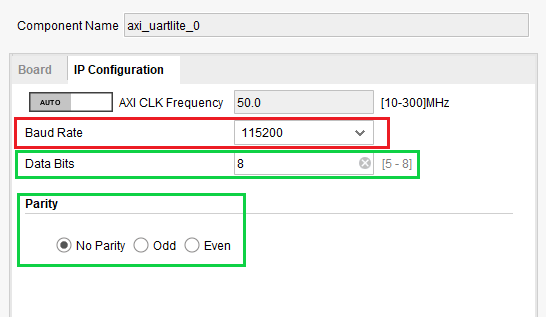
\includegraphics{./../../img/Images/uartlite_ip_configuration_col}
  \caption{IP configuration with {\color{Red}Baud Rate} and {\color{Green} bits} definition}
  \label{ip_config}
\end{figure}

\begin{figure}[h]
  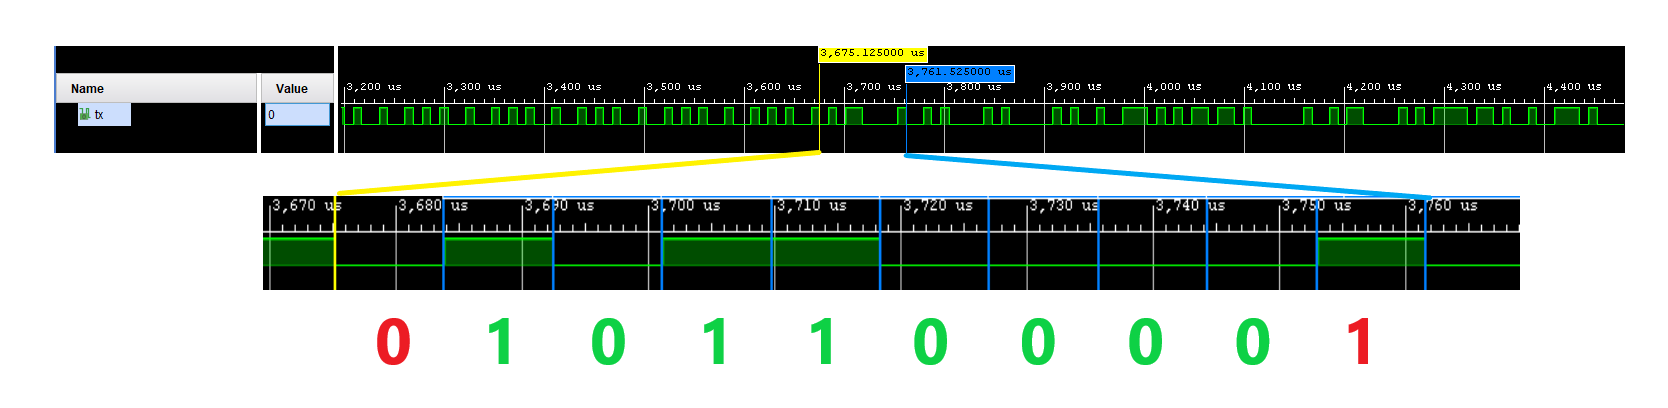
\includegraphics[width=\textwidth]{./../../img/Images/uart_tx_0x0d}
  \caption{ 0x0d ( \textcolor{Green}{0000\_1101} in binary ) in the tx channel waveform with \textcolor{Red}{start} and \textcolor{Red}{end} bits}
  \label{0x0d_waveform}
\end{figure}


{\color{Blue}\subsection{Decoding Software}}
%explain cose used for deconding
After analysing the signals transmitted by the uartlite and after understanding their encoding, we wrote in the {\bf Verilog file} of the testbench some lines of code in order to make {\bf automatic} the {\bf decoding of the output} and, at the same time, write it on a text file.
\newline

All the {\bf read bits} are saved in {\bf three register} variables ({\verb+start_sig+}, {\verb+buffer+} and { \verb+end_sig+}, respectively) and cleaned a clock’s cycle after being writtten or, for the { \verb+end_sig+}, at the beginning of the always block using value Z for one bit variable and 0 for the buffer.
\newline

The {\bf assigning} and the {\bf checking} of the tx’s values occur at the {\bf positive edge} of the { \verb+clk_baud+}. This is because we noticed that the bit changing is aligned with that clock.
\newline
